% Sångtext till VN:s sångbok 2010.

% Denna fil kan användas som sådan, bara verserna,
% namnen och annan rådata behöver bytas ur fälten.
% Tecknet "%" markerar en kommentar som helt och 
% hållet ignoreras av programmet som läser filen.

\beginsong{In blåmåla plåtbåt}[ 		% Börja sången här
	by={Anders Teir},					% Författare
	sr={Proud Mary},					% Melodi
	index={Emel for åp ped ti Öjen}, 						% Alternativa
	index={Tusan, jäken, köm a stuli nöulon}]						% sångnamn
	

\beginverse*						% Börja vers
Emel for åp ped ti Öjen
markan i in burk å e mäitspö me.
Åp strandän bräivär slussin
stal an se in roddbåt
for ut i Kaskusånde å sku buri mäit.
Men höfstup vort an longvåt
i in blåmåla plåtbåt.
Tusan, jäken
köm a stuli nöulon?
\endverse							% Sluta vers

\beginverse*						% Börja vers
Emel kom ti plomp i fjälin
feg in rekti kalsup så an vela spy.
He smaka cellulosa,
smaka värr en dynjon.
Emel for ti båten som i seck med bly.
Men höfstup kom e titåt
in blåmåla plåtbåt.
Tusan, jäken
tennar kommer Folkline!
\endverse							% Sluta vers

\beginverse*						% Börja vers
Folkline tjuta me sirenin
å Emel dro di opp som in arin mört
Så tömd di ur an vattne,
å tömd i an na välkan.
Emel liva i å va itt ens na trött.
Ä notstup for an häimåt
i in blåmåla plåtbåt.
:,: Tusan, jäken
köm a stuli nöulon? :,:
\endverse							% Sluta vers
\endsong							% Sluta sång

\begin{figure}[!b]
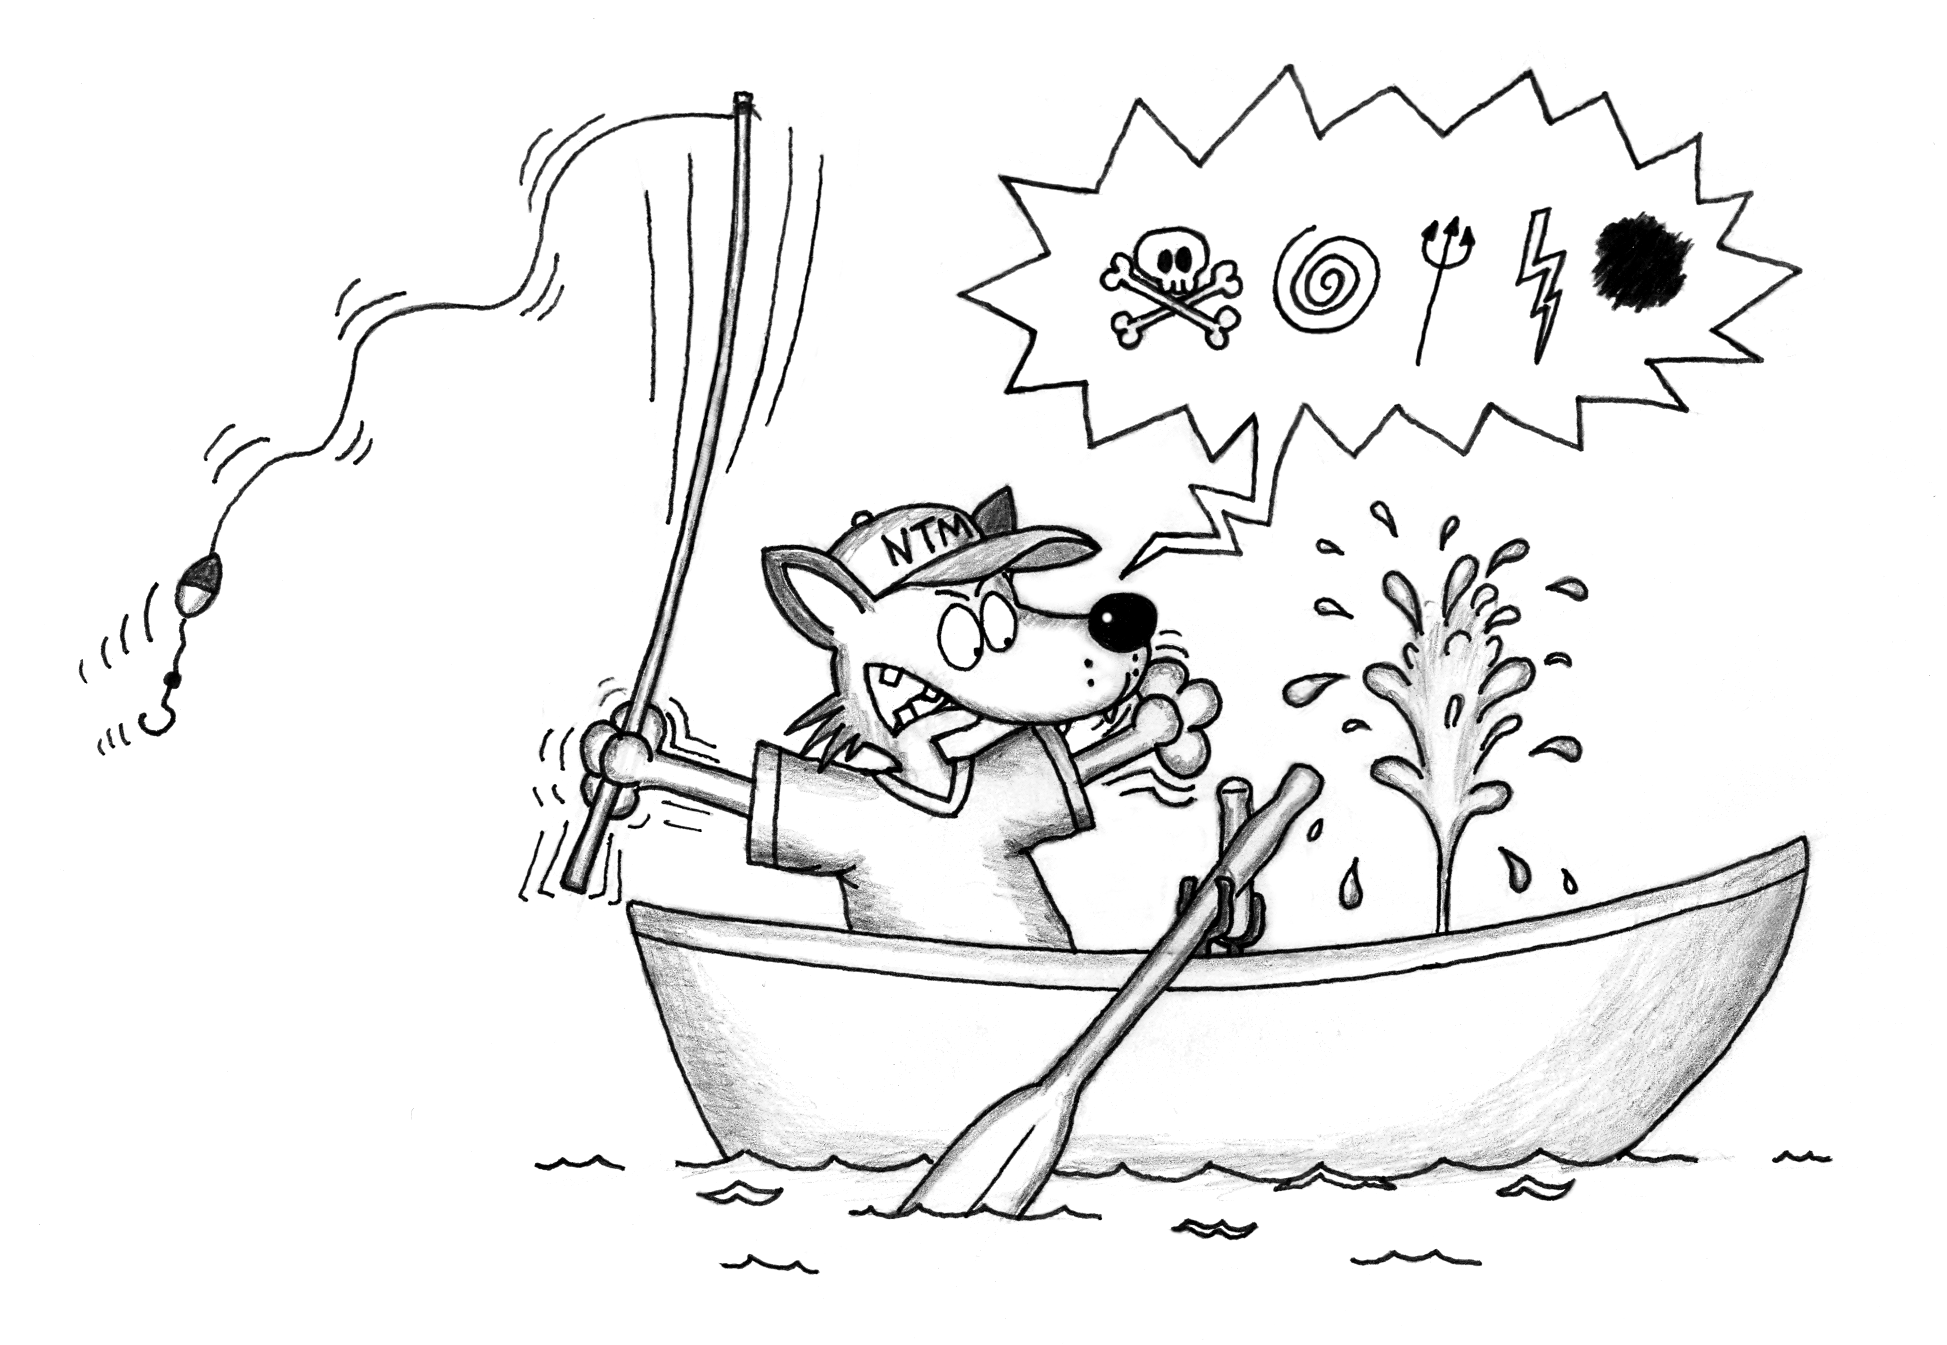
\includegraphics[scale=.4]{../bilder/in_blamala_platbat.png} 
\end{figure}
